\documentclass[letterpaper,10pt,oneside]{article}

\usepackage[style=authoryear, backend=biber, natbib=true]{biblatex}

\bibliography{mybib}

\usepackage{graphicx}
\graphicspath{ {/Users/jacksonwills/Documents/Fitz_Research/Report} }

\usepackage{amsmath, amssymb, amsfonts, bm, mathtools}
\usepackage{hyperref}


\title{System Modeling and Control of the Furuta Pendulum}
\author{Jackson Wills}



\begin{document}

\maketitle

\tableofcontents

Random citation \cite{SWINGUP} embeddeed in \citet{SWINGUP} text \cite{DYNAMICS}

In this paper, \citep{SWINGUP} the dynamics of the Furuta Pendulum are simulated and the system is given reasonable parameters and controlled using linear full-state feedback control. The Furuta Pendulum was developed by a man named Katsuhisa Furuta at the Tokyo Institute of Technology in 1992 \cite{DYNAMICS}. The device consists of an motor which can rotate a beam in the horizontal plane. Attatched to that beam is a pendulum which is free to rotate in the vertical plane - see figure \ref{fig:diagram}.


\begin{figure}
  \centering
  % 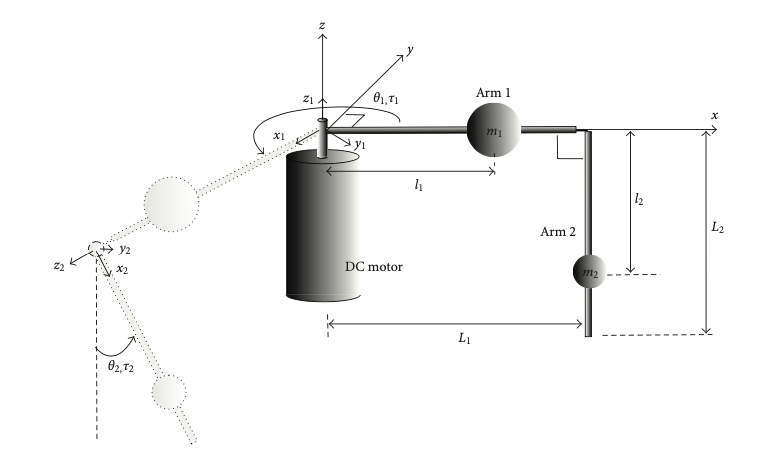
\includegraphics[scale = .6]{FurutaDiagram.png}
  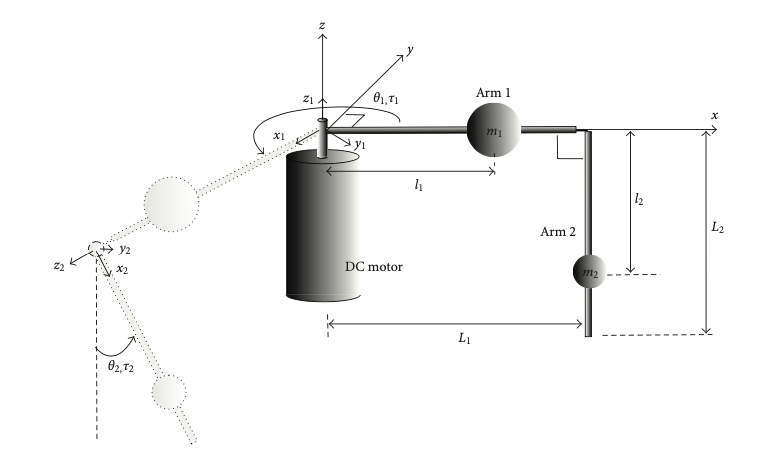
\includegraphics[width=0.9\textwidth]{FurutaDiagram}
  \caption{A diagram of the Furuta Pendulum \cite{DYNAMICS}}
  \label{fig:diagram}
\end{figure}


The first thing to do is to get equations of motion which accurately model the system. These equations were derived largely with the help of Cazzolato and Prime \cite{DYNAMICS}. The equations of motion were found to be \\


\begin{multline}
  0 = - 2.0 J_{2xx} \dot{\theta}_{1} \dot{\theta}_{2} \sin{\left(\theta_{2}{\left(t \right)} \right)} \cos{\left(\theta_{2}{\left(t \right)} \right)} + 2.0 J_{2yy} \dot{\theta}_{1} \dot{\theta}_{2} \sin{\left(\theta_{2}{\left(t \right)} \right)} \cos{\left(\theta_{2}{\left(t \right)} \right)}
        \\
   + 1.0 L_{1} l_{2} m_{2} \ddot{\theta}_{2} \cos{\left(\theta_{2}{\left(t \right)} \right)} - 1.0 L_{1} l_{2} m_{2} \dot{\theta}_{2}^{2} \sin{\left(\theta_{2}{\left(t \right)} \right)} + b_{1} \dot{\theta}_{1} + \\ 2.0 l_{2}^{2} m_{2} \dot{\theta}_{1} \dot{\theta}_{2} \sin{\left(\theta_{2}{\left(t \right)} \right)} \cos{\left(\theta_{2}{\left(t \right)} \right)} - \tau_{1}
    \\
    + \ddot{\theta}_{1} \left[1.0 J1zz + 1.0 J_{2xx} \cos^{2}{\left(\theta_{2}{\left(t \right)} \right)} + 1.0 J_{2yy} \sin^{2}{\left(\theta_{2}{\left(t \right)} \right)} + 1.0 L_{1}^{2} m_{2} \sin^{2}{\left(\theta_{2}{\left(t \right)} \right)}
      \right.
      \\
      \left.
     + 1.0 L_{1}^{2} m_{2} \cos^{2}{\left(\theta_{2}{\left(t \right)} \right)} + 1.0 l_{1}^{2} m_{1} + 1.0 l_{2}^{2} m_{2} \sin^{2}{\left(\theta_{2}{\left(t \right)} \right)}\right]
\end{multline}

\begin{align}
  x &= \left( 2 + \frac{1}{3} \right) \label{eq:important}\\
  y &= 4x
\end{align}

Some radom text. See \eqref{eq:important} for blah.

$0 = 1.0 J_{2zz} \ddot{\theta}_{2} + 1.0 L_{1} l_{2} m_{2} \ddot{\theta}_{1} \cos{\left(\theta_{2}{\left(t \right)} \right)} + b_{2} \dot{\theta}_{2} + g l_{2} m_{2} \sin{\left(\theta_{2}{\left(t \right)} \right)} + 1.0 l_{2}^{2} m_{2} \ddot{\theta}_{2} - \tau_{2} + \dot{\theta}_{1}^{2} \left(1.0 J_{2xx} \sin{\left(\theta_{2}{\left(t \right)} \right)} \cos{\left(\theta_{2}{\left(t \right)} \right)} - 1.0 J_{2yy} \sin{\left(\theta_{2}{\left(t \right)} \right)} \cos{\left(\theta_{2}{\left(t \right)} \right)} - 1.0 l_{2}^{2} m_{2} \sin{\left(\theta_{2}{\left(t \right)} \right)} \cos{\left(\theta_{2}{\left(t \right)} \right)}\right)$


These equations were then linearized about $\theta_{1} = \pi$ and $\theta_{2} = 0.$ \\
The goal of the control law was to keep $\theta_{1}$ at  $\pi$, assuming the system started near $\pi$.\\

A linear full-state feedback control law was implemented and the resulting gain matrix is: \\

$ k =
\begin{bmatrix}
  8.53 &
  -15.90 &
  -3.66 &
  -0.97
\end{bmatrix}$

\begin{align}
  k = \left[\begin{array}{cccc}
  8.53 &
  -15.90 &
  -3.66 &
  -0.97
  \end{array}\right]
\end{align}


\section{New section}
\subsection{New Subsection}

\newpage


\printbibliography

\newpage
\appendix
\section{New Section}


\end{document}
